% ---------------------------------------------------------------------
% HEADER
% Formålet med å legge header til et eget dokument er å garantere at
% oppsettet av dokumentene er likt for alle løsningsforslagene.
% I headeren skjer følgende:
% (1) Dokumentet blir startet
% (2) Pakker blir importert
% ---------------------------------------------------------------------
% ---------------------------------------------------------------------
% HEADER
% Formålet med header er å importere de samme pakkene i alle dokumentene.
% ---------------------------------------------------------------------

% Sett opp dokumentet. Her kan 'twoside' brukes for printing
\documentclass[12pt, a4paper]{article}

% Vi trenger utf-8 for å bruke norske bokstaver: Æ, Ø, Å
\usepackage[utf8]{inputenc}

% Vi setter babel til norsk, da får dokumentegenskaper norske titler
\usepackage[norsk]{babel}

% For å kunne bruke grafikk
\usepackage{graphicx}
\newcommand{\figwidth}{0.75}

% Matematikkpakker fra AMS - American Mathematical Society
\usepackage{amsmath, amsthm, amsfonts, amssymb, mathtools}

% For eventuelle linker, e.g. \href{URL}{text}
\usepackage{hyperref}

% For headers og footers med eventuell logo
\usepackage{fancyhdr}

% Sett marginer manuelt
\usepackage[top = 3cm, left = 3cm, right = 3cm, bottom = 3cm]{geometry}

% For enkle lister, nyttig for oppgave a), b), c), ...
\usepackage[sharp]{easylist}

% Dersom flere kolonner er ønskelig i deler av dokumentet
\usepackage{multicol}

% For luft mellom paragrafer
\usepackage{parskip}

% For logikk assosiert med logoer
\usepackage{ifthen}

% For å finne totalt antall sider
\usepackage{lastpage}

% Annet
\usepackage{enumitem}

\usepackage{polynom}% Polynomer
\polyset{style=C, div=:}

\usepackage{systeme}% Likningssystemer

% Kan brukes når noe stryker ut noe, f.eks 1/n * n, her kan man ta \frac{1}{\cancel{n}} * \cancel{n}
\usepackage{cancel}

\usepackage{tikz}

% ---------------------------------------------------------------------
% DOKUMENTVARIABLER
% ---------------------------------------------------------------------
\newcommand{\fagkode}{R1}
\newcommand{\semesteraar}{høsten 2018}
\newcommand{\forfatter}{Sindre S.H. og Tommy O.}
\newcommand{\dokumenttittel}{Løsningsforslag -- Eksamen \fagkode, \semesteraar}

% Set til 'true' og oppgi logo dersom du vil bruke en logo
\newboolean{bruklogo}
\setboolean{bruklogo}{false}
\newcommand{\logonavn}{}


% ---------------------------------------------------------------------
% SETUP
% Formålet med å legge setup til et eget dokument å garantere at headers,
% footers, og øverste del av dokumentet er likt for alle
% løsningsforslagene.
% ---------------------------------------------------------------------
% ---------------------------------------------------------------------
% HEADER
% Formålet med setup er at dokumentene ser rimelig like ut.
% ---------------------------------------------------------------------


% ---------------------------------------------------------------------
% Alternativ font. Kommentert ut fordi Computer Modern (default) er pen
%\usepackage{kmath,kerkis}
%\usepackage[T1]{fontenc}
% ---------------------------------------------------------------------


% ---------------------------------------------------------------------
% Sett opp headers og footers
\ifthenelse{\boolean{bruklogo}}{
% Dersom logo skal brukes, sett logoen oppe til høyre med bredde 4 cm
	\rhead{\includegraphics[width=3.5cm]{\logonavn}}
}{
% Dersom logo ikke skal brukes, sett tom header
	\rhead{}
} 
\rfoot{\thepage}
\cfoot{}
\lhead{}
\lfoot{{\scriptsize Forbedringsforslag? Bidra på \url{https://github.com/tommyod/matte_eksamener_VGS}.}}
\renewcommand{\headrulewidth}{0pt}
% ---------------------------------------------------------------------


% ---------------------------------------------------------------------
% To streker under svaret
\def\answer#1{\underline{\underline{#1}}}
% ---------------------------------------------------------------------


% ---------------------------------------------------------------------
% Start selve dokumentet
% ---------------------------------------------------------------------

\begin{document}
\pagestyle{fancy}
{\bfseries \Large \dokumenttittel} \\
{ \footnotesize Laget av \forfatter 
	\hfill Sist oppdatert: \today 
	\hfill Antall sider: \pageref*{LastPage}}
\hrule
\vspace{1em}
\begin{center}
\fbox{\fbox{\parbox{.90\textwidth}{
	Dette dokumentet er open-source;
	alle kan bidra til å gjøre det bedre.
	Dersom du finner skrivefeil, matematiske feil, eller ser at forklaringene kan være bedre: ikke nøl med å sende inn en endring. 
	Du kan finne siste versjon, og bidra, på GitHub, se:
	\url{https://github.com/tommyod/matte_eksamener_VGS}
}}}
\end{center}


% ---------------------------------------------------------------------
% DOKUMENTSTART - Skriv løsningsforslaget nedenfor
% ---------------------------------------------------------------------	
\section*{Del 1 - uten hjelpemidler}
\subsection*{Oppgave 1}
\begin{easylist}[enumerate]
\ListProperties(Style2*=,Numbers=a,Numbers1=l,FinalMark={)})
# Vi deriverer ledd for ledd, og får at
\begin{equation*}
	f'(x) = \answer{2x + 2 + e^x}.
\end{equation*}

# Vi bruker her produktregelen for derivasjon og får at
\begin{align*}
	g'(x) &= \left(x^2\right)'\ln x + x^2(\ln x)' 	\\
	&= 2x \ln x + x^2 \frac{1}{x} \\
	&= 2x \ln x + x \\
	&= \answer{x(2\ln x + 1)}.
\end{align*}


# Her har vi to muligheter, og vi viser begge.
\textbf{Alternativ 1 - Omskrivning til produktregelen:} \\
Vi omskriver $ h(x) $ ved hjelp av potensregler til $h(x) = (x-1)e^{-(2x+1)}$.
Videre merker vi oss at av kjerneregelen at
\begin{equation*}
	\left(e^{-(2x+1)}\right)'=-2e^{-(2x+1)}.
\end{equation*}
Av produktregelen ser vi da at
\begin{align*}
h'(x) &= (x-1)'e^{-(2x+1)}+(x-1)\left(e^{-(2x+1)}\right)'  \\
&= 1\cdot e^{-(2x+1)} - 2(x-1)e^{-(2x+1)} \\
&= (1-2(x-1))e^{-(2x+1)} \\
&= \answer{(3-2x)e^{-(2x+1)}}.
\end{align*}

\textbf{Alternativ 2 - Derivasjon ved hjelp av kvotientregelen:}\\
Vi ser at
\begin{align*}
	(x-1)' &= 1\\
	\left(e^{2x+1}\right)' &= 2e^{2x+1}. \tag{kjerneregelen}
\end{align*}
Av kvotientregelen ved derivasjon har vi da at
\begin{align*}
	h'(x) &= \frac{(x-1)'e^{2x+1}-(x-1)\left(e^{2x+1}\right)'}{\left(e^{2x+1}\right)^2} \\
	&= \frac{1\cdot e^{2x+1} - (x-1)2e^{2x+1}}{e^{2(2x+1)}
	} \\
	&= \frac{e^{2x+1}(1-(x-2))}{e^{2(2x+1)}}\\
	&= \answer{\frac{3-2x}{e^{2x+1}}},
\end{align*}
og dette er samme svar som i første alternativ.
Fordelen med å skrive om til produktregelen er at vi får mindre regler å huske på, ulempen er at utregningene potensielt kan være mer krevende.

\end{easylist}



\subsection*{Oppgave 2}
\begin{easylist}[enumerate]
\ListProperties(Style2*=,Numbers=a,Numbers1=l,FinalMark={)})
# Vi merker oss at
\begin{equation*}
	e^{2x}+7e^x -8 = \left(e^ x\right)^2 + 7\left(e^ x\right) - 8 =0.
\end{equation*}
Dette betyr at vi kan løse en andregradsligning med hensyn på $e^x$. 
Vi viser her to måter å løse ligningen på.\\
\textbf{Alternativ 1 - ved hjelp av abc-formelen:} \\
Ved abc-formelen ser vi at
\begin{equation*}
	e^x = \frac{-7\pm \sqrt{7^2-4\cdot1\cdot(-8)}}{2\cdot1}	 
	= \frac{-7\pm \sqrt{81}}{2} 
	= \frac{-7\pm 9}{2}.
\end{equation*}
\textit{Alternativ 2 - uten abc-formelen}\\
Ettersom  $ 8(-1)=-8 $ og $ 8-1=7 $, har vi at $(e^x +8)(e^x-1)=0$.

Både \textbf{Alternativ 1} og \textbf{Alternativ 2} gir løsningene
\begin{equation*}
e^x = 1 
\quad\vee\quad 
e^x = -8.
\end{equation*}
Siden $e^x > 0$ for alle verdier av $x$, står vi bare igjen med løsningen $e^x=1$:
\begin{equation*}
	\ln e^x = \ln 1 \quad \Rightarrow \quad \answer{x = 0}.
\end{equation*}


# Ved hjelp av logaritmeregler omskriver vi ligningen til
\begin{equation*}
	\ln \left(\frac{x^2-5x-1}{3-2x}\right)=0.
\end{equation*}
Videre har vi at
\begin{align*}
	e^{\ln \left(\frac{x^2-5x-1}{3-2x}\right)}&=e^0 \\
	\frac{x^2-5x-1}{3-2x} &= 1 \\
	x^2-5x-1 &= 3-2x \\
	x^2-3x-4 &= 0
\end{align*}
Vi faktoriserer uttrykket, enten ved hjelp av abc-formelen, eller ved å merke oss at $ (-4)1 =-4 $ og $ -4+1=-3 $, og dette leder til
\begin{equation*}
	x^2-3x-4 = (x-4)(x+1)=0
\end{equation*}
Ettersom $ x=4 $ fører til at vi tar logaritmen av et negativt tall (og dette kan vi ikke gjøre\footnote{
Vi kan ikke ta logaritmen av et negativt tall $x$, fordi logaritmen er invers av eksponentialfunksjonen og svarer på spørsmålet ``Hva må $e$ opphøyes i for å få $x$?''. 
Med andre ord: vi kan ikke ta logaritmen av et negativt tall $x$, fordi det finnes ingen $y$ som løser $e^y = x$ når $x \leq 0$.
}), står vi bare igjen med $\answer{ x=-1 }$ som gyldig løsning.
\end{easylist}

\subsection*{Oppgave 3}
\begin{easylist}[enumerate]
	\ListProperties(Style2*=,Numbers=a,Numbers1=l,FinalMark={)})
	# Vi bruker regelene for addisjon og multiplikasjon av vektorer med skalarer og får at
	\begin{align*}
		2\vec{b}-3\vec{a} &= 2[-5, 3] - 3[2, 3]	\\
		&= [-10, 6]-[6, 9] = \answer{[-16, -3]}.
	\end{align*}
	
	
	# Vi bruker formelen for lengden av en vektor og ser at
	\begin{equation*}
		|\vec{a}| = \sqrt{2^2 + 3^2} = \sqrt{13}.
	\end{equation*}
	Ettersom $ \sqrt{13}<\sqrt{16}=4 $ er $ |\vec{a}| $ mindre enn 4.


	# En stump vinkel har negativ cosinusverdi, en rett vinkel har cosinusverdien 0 og en spiss vinkel har positiv cosinusverdi. 
	Cosinus av vinkelen $\theta$ mellom to vektorer $\vec{a}$ og $\vec{b}$ er gitt av formelen
	\begin{equation*}
		 \cos \left(  \theta \right) = \frac{\vec{a}\cdot\vec{b}}{|\vec{a}||\vec{b}|},
	\end{equation*}
	og gitt vektorene i oppgaven ser vi at
	\begin{equation*}
		|\vec{a}|, |\vec{b}| > 0\quad,\quad\vec{a}\cdot\vec{b}=2(-5)+3\cdot3=-1
		\quad \Rightarrow\quad
		 \cos \left(  \theta \right) <0.
	\end{equation*}
	Ettersom telleren er negativ og telleren er positiv, må cosinus av vinkelen være negativ---da er $\theta$ en \answer{stump vinkel}.
\end{easylist}


\subsection*{Oppgave 4}
\begin{easylist}[enumerate]
	\ListProperties(Style2*=,Numbers=a,Numbers1=l,FinalMark={)})
	# Vi bruker polynomdivisjon og ser at \\
	\polylongdiv{x^3+6x^2-x-30}{x-2}
	
	
	# Vi faktoriserer ved hjelp av abc-formelen eller ved å merke oss at $ 3\cdot5 = 15 $ og $ 3+5=8 $. Da har vi at
	\begin{equation*}
		x^2+8x+15 = (x+3)(x+5),
	\end{equation*}
	og dermed får vi at
	\begin{equation*}
		x^3+6x^2-x-30=  \answer{(x+3)(x+5)(x-2)},
	\end{equation*}
	og vi har dermed faktorisert  $f(x)$ i lineære faktorer.
	# At $ -2 f(x)\geq 0 $ er ekvivalent med at $ f(x)\leq 0 $, dette ser vi dersom vi ganger begge sider med $-2$. 
	Vi setter opp et fortegnsskjema for å løse denne ulikheten:
		\begin{figure}[ht!]
		\centering
		\begin{tikzpicture}[scale=2]	
	% Start
		\draw[color=black] (0,0.25) -- (0,-1.75);
		
		\node[anchor=east] at (0,0) { $(x+3)$};  
	    \node[anchor=east] at (0,-0.5) { $(x+5)$};  		
	  	\node[anchor=east] at (0,-1) {$(x-2)$};       	
	  	\node[anchor=east] at (0,-1.5) {$f(x)$};   
	
	% Til -5
		\node[anchor=south] at (1,0.25) { $-5$};    		
		\draw[color=black] (1,0.25) -- (1,-1.75);	
		
  		\draw[dashed,color=black] (0,0) -- (1,0);
  		\draw[dashed,color=black] (0,-0.5) -- (1,-0.5);
  		\filldraw (1,-0.5) circle[radius=1pt] ;  
  		\draw[dashed,color=black] (0,-1) -- (1,-1);
  		\draw[dashed,color=black] (0,-1.5) -- (1,-1.5);
  		\filldraw (1,-1.5) circle[radius=1pt] ;  

	% Til -5
		\node[anchor=south] at (2,0.25) { $-3$};    		
		\draw[color=black] (2,0.25) -- (2,-1.75);	
		
		\draw[dashed,color=black] (1,0) -- (2,0);
		\draw[color=black] (1,-0.5) -- (2,-0.5);
		\filldraw (2,0) circle[radius=1pt] ;  
		\draw[dashed,color=black] (1,-1) -- (2,-1);	
		\draw[color=black] (1,-1.5) -- (2,-1.5);
		\filldraw (2,-1.5) circle[radius=1pt] ;  		
	
	% Til 2
		\node[anchor=south] at (3,0.25) { $2$};    		
		\draw[color=black] (3,0.25) -- (3,-1.75);	
		
		\draw[color=black] (2,0) -- (3,0);
		\draw[color=black] (2,-0.5) -- (3,-0.5);
		\filldraw (3,-1) circle[radius=1pt] ;  
		\draw[dashed,color=black] (2,-1) -- (3,-1);			
		\draw[dashed, color=black] (2,-1.5) -- (3,-1.5);
		\filldraw (3,-1.5) circle[radius=1pt] ;  			

	% Slutt	
		\draw[color=black] (4,0.25) -- (4,-1.75);	
		\draw[color=black] (3,0) -- (4,0);
		\draw[color=black] (3,-0.5) -- (4,-0.5);
		\draw[color=black] (3,-1) -- (4,-1);		
		\draw[color=black] (3,-1.5) -- (4,-1.5);
		\filldraw (3,-1.5) circle[radius=1pt] ;  			
		\end{tikzpicture}
	\end{figure}

Av figuren ser vi at $ f(x)\leq 0 $ når $\answer{x\leq -5 \, \vee \, -3\leq x \leq 2}$.
\end{easylist}



\subsection*{Oppgave 5}
Vi definerer følgende hendelser.
\begin{align*}
	A &= \text{Mann}\quad&\bar A &= \text{Kvinne}	\\
	B &= \text{Kjøper edelgran}\quad &\bar B &= \text{Kjøper vanlig gran}
\end{align*}
Basert på oppgaveteksten har vi at
\begin{align*}
	P(A) &= 70 \, \% \quad& P(\bar A) &= 30 \, \%	\\
	P(B \mid A) &=60 \, \%\quad & P( B \mid \bar A) &= 40 \, \% 
\end{align*}

\begin{easylist}[enumerate]
\ListProperties(Style2*=,Numbers=a,Numbers1=l,FinalMark={)})
#  Av formelen for total sannsynlighet har vi at
\begin{align*}
	P(B) &= P(A)P(B \mid A)+P(\bar A)P(B \mid \bar A) \\
	&= 0.7 \cdot 0.6 + 0.3 \cdot 0.4 = \answer{0.54}.
\end{align*}
Det er altså 54 \% sannsynlighet for at første solgte tre er en edelgran.


# Spørsmålet i oppgaven er det samme som å spørre hva sannsynligheten er for at kjøperen av et tre er en kvinne, gitt at treet er en edelgran. 
Av Bayes' setning har vi at
\begin{equation*}
		P(\bar A \mid B)	= \frac{P(B \mid \bar A)\cdot P(\bar A)}{P(B)} 
		= \frac{0.4\cdot 0.3}{0.54} 
		= \frac{12}{54}
		= \frac{2}{9}
\end{equation*}
Sannsynligheten er altså $ \answer{2/9 \approx 22.2 \, \%}$ for at lotterivinneren er en kvinne.
\end{easylist}



\subsection*{Oppgave 6}
Skal $ f(x) $ være kontinuerlig, må $\lim_{x^\pm \to a} f(x) =f(a)$.
Sagt med ord må funksjonen $f(x)$ gå mot samme verdi når $x$ nærmer seg $a$, både fra venstre, fra høyre og i selve punktet $a$.
I vårt tilfelle er det tilstrekkelig å sørge for at $ f(a) $ får samme verdi ved begge tilfeller av funksjonsuttrykkene for $ f(x) $.
Vi ser at
\begin{align*}
	2a^2 - 3a - 2 &= a^2 +a + 3 = (a-5)(a+1)=0 \\
	a^2 -4a-5 &= 0
\end{align*}
Derfor er funksjonen$ f(x) $ kontinuerlig når \answer{$a = 5 \, \vee \,  a=-1$}.



\subsection*{Oppgave 7}
\begin{easylist}[enumerate]
	\ListProperties(Style2*=,Numbers=a,Numbers1=l,FinalMark={)})
	# Vi bruker kjernereglen på andre ledd, og deriverer $g'(x)$ slik at vi får
	\begin{equation*}
		g'(x) = 1 - \left(2\ln(x^2+3)\right)' = 1 - \frac{4x}{x^2+3} =
		\frac{x^2+3}{x^2+3} - \frac{4x}{x^2+3} = \answer{\frac{x^2-4x+3}{x^2+3}}.
	\end{equation*}


	# I ett toppunkt eller bunnpunkt må vi ha $g'(x) = 0$.
	Vi faktoriserer telleren og løser $g'(x) = 0$:
	\begin{equation*}
		\frac{(x-1)(x+3)}{x^2+3}= 0 
		\quad \Rightarrow \quad
		x= 1 \, \vee \, x= 3
	\end{equation*}
	Ved å sette opp et fortegnsskjema (ikke vist her, se gjerne oppgave 4c for en påminnelse) finner vi at \answer{$x=1$ er $x$-verdien til et maksimalpunkt}, og at \answer{$x=3$ er $x$-verdien til et minimumspunkt}.
	
	
	# Et vendepunkt oppstår når $g''(x)$ endrer fortegn, altså når $g''(x)$ går fra å være positiv til negativ, eller motsatt\footnote{Funksjonen $f(x) = x^4$ har ingen vendepunkter, selv om $f''(x) = 0$ når $x=0$. Dette er fordi $f''(x) = 0$ ikke endrer fortegn. Funksjonen er alltid konveks.}.
	Vi finner den dobbelderiverte ved hjelp av kvotientregelen.
	\begin{equation*}
		g'(x)	= \frac{\left(x^2-4x+3\right)'\left(x^2+3\right)-\left(x^2-4x+3\right)\left(x^2+3\right)'}{\left(x^2+3\right)^2}
	\end{equation*}
	Nevneren er aldri negativ, så $g''(x)$ endrer ikke fortegn på grunn av endring i fortegn i nevneren.
	Vi forenkler telleren og ser at
	\begin{gather*}
		(2x-4)(x^2+3)-2x(x^2-4x+3) = \\
		2x^3+6x-4x^2-12-2x^3+8x^2-6x = \\
		4x^2 - 12
	\end{gather*}
	Telleren endrer fortegn når $4x^2 - 12 = 4(x - \sqrt{3})(x + \sqrt{3})$ endrer fortegn.
	Altså har $g(x)$ vendepunkter, eller infleksjonspunkter, når
	\begin{equation*}
		\answer{x = \sqrt{3} \quad \vee \quad x=-\sqrt{3}}.
	\end{equation*}

\end{easylist}


\subsection*{Oppgave 8}
\begin{easylist}[enumerate]
	\ListProperties(Style2*=,Numbers=a,Numbers1=l,FinalMark={)})
	# TODO :)
	# TODO :)
	# TODO :)
\end{easylist}



\clearpage 
\section*{Del 2 - med hjelpemidler}

\subsection*{Oppgave 1}
La $X$ være antall gule blomster.
Da er $X$ binomisk fordelt, fordi fargen til hver blomst er uavhengig av de andre, sannsynligheten for gul er alltid $p = 0.4$, og det er kun to utfall per blomst---enten gul eller rød.

\begin{easylist}[enumerate]
	\ListProperties(Style2*=,Numbers=a,Numbers1=l,FinalMark={)})
	# Vi lar $X$ være antall gule blomster, da er $X$ binomisk fordelt med $n=10$ og $p=0.4$. 
	Sannsynligheten for at $X=5$ blir da
	\begin{equation*}
		P(X = 5) = \binom{n}{k} p^k (1-p)^{n-k} = 
		\binom{10}{5} 0.4^5 0.6^{5} \approx 0.2007 = \answer{20.1 \, \%},
	\end{equation*}
	der vi henter svaret fra Geogebras sannsynlighetskalkulator i praksis.
	
	
	# Dette er $P(X > 5)$, og fra sannsynlighetskalkulatoren i Geogebra får vi
	\begin{equation*}
		P(X > 5) \approx 0.1662 = \answer{16.6 \, \%} .
	\end{equation*}
	# Her kan det være nyttig å snu litt på problemstillingen.
	Vi har 10 plasser $P_1, P_2, \dots, P_{10}$ totalt, og vi må trekke ut fire plasser til de gule blomstene.
	Da er plasseringen til de andre blomstene også bestemt.
	Rekkefølgen har ikke noe å si, fordi $\{ P_3, P_5, P_6, P_9 \}$ eksempelvis er det samme som $\{ P_6, P_5, P_3, P_9 \}$.
	Spørsmålet er med andre ord ``På hvor mange måter kan vi velge 4 plasser for de gule blomstene, nå rekkefølgen er uviktig?''.
	Dette er antall kombinasjoner, og svaret blir $\binom{10}{4} = \answer{210}$.
	I Geogebra skriver man \verb|nCr(10, 4)| i CAS.
	
	Legg også merke til at dette spørsmålet er det samme som å spørre ``På hvor mange måter kan vi velge 6 plasser for de røde blomstene, nå rekkefølgen er uviktig?'', og at svaret da blir $\binom{10}{6} = \answer{210}$.
\end{easylist}

\subsection*{Oppgave 2}
\begin{easylist}[enumerate]
	\ListProperties(Style2*=,Numbers=a,Numbers1=l,FinalMark={)})
	#  Siden $ CB|| AE $ og $ \angle BCD $ og $ \angle AED $ er på motsatt side av $ AE $, har vi at $ \angle BCD = \angle AED $. 
	
	
	# Vi argumenterer punkt for punkt:
	\begin{itemize}
		\item Vi har forklart i oppgave a) at $  \angle BCD = \angle AED$
		\item Siden $ \angle ADE $ og $ \angle BDC $ er på motsatt side av $ AE $, og begge vinklene deler linja $ AB $, er $ \angle BCD = \angle AED $ 
		\item Fordi trekantene har to samsvarende vinkler, er $ \triangle DBC \sim \triangle AED $ (formlike).
	\end{itemize}
	
	
	# $ \triangle AEC $ består blant annet av vinklene $ ACD $ og $ AED. $ Siden 
	\begin{equation*}
		\angle AED = \angle BCD = \alpha = ACD,
	\end{equation*}
	 har $ \triangle AEC $ to like vinkler og er derfor likebeint.
	 
	 
	# Siden $ \triangle DBC \sim \triangle AED $ er forholdet mellom to samsvarande sider i trekantene likt. 
	Vinkel $ \angle AED$ og $ \angle BCD $ utspenner respektivt linjene $ AD $ og $ DB $, mens $ \angle ADE$ og $ \angle CDB $ utspenner respektivt linjene $ AE $ og $ a$. 
	Da har vi at
	\begin{equation*}
		\frac{AD}{DB}= \frac{AE}{a}
	\end{equation*}
	Siden $ \triangle ACE $ er likebeint er $ AE=b $:
	\begin{equation*}
		\frac{AD}{DB}= \frac{b}{a}
	\end{equation*}
	Som var det vi skulle vise.


	# Siden $ c=10 $, har vi at $ DB=10-AD $. 
	Dermed kan vi bruke forholdet fra opg. d) til å løse en ligning med hensyn på $ AD $. 
	Likningen er løst i CAS:
	\begin{figure}[h]
		\centering
		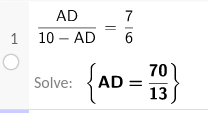
\includegraphics[scale=0.6]{figs/D2opg2e.png}
		\caption{Ligning for $ AD $ løst i CAS i Geogebra.}
	\end{figure}
\end{easylist}



\subsection*{Oppgave 3}
\begin{easylist}[enumerate]
	\ListProperties(Style2*=,Numbers=a,Numbers1=l,FinalMark={)})
	# Linjen $\ell$ er gitt av
	\begin{equation*}
	\ell(k) = A + \vec{AB} k = (3, 0) + \left[ (5, 5) - (3, 0) \right] k = (2k+3, 5k).
	\end{equation*}
	# Se figur \ref{fig:del2_oppg3} for en tegning av grafen, utført med kommandoen \\
	\verb|Kurve(<Uttrykk>, <Uttrykk>, <Parametervariabel>, <Start>, <Slutt>)|,\\
	samt linjen $\ell(k)$.
	
	
	# Linja fra $A$ til $B$ er gitt av $\vec{AB} = (2, 5)$.
	Tangenten er gitt av $T(t) = r'(t) = (1, 2t)$.
	Disse to vektorene er parallelle dersom der finnes en $z$ slik at
	\begin{equation*}
	\begin{pmatrix}
	2 \\
	5
	\end{pmatrix} z =
	\begin{pmatrix}
	1 \\
	2t
	\end{pmatrix}.
	\end{equation*}
	Dette er et likningssett med 2 ukjente og 2 likninger, og løsningen er $z = 1/2$ og $t = 5/4$.
	Setter vi $t = 5/4$ inn i $r(t)$ får vi punktet 
	\begin{equation*}
	\answer{\begin{pmatrix}
		9/4 \\
		57/6
		\end{pmatrix}},
	\end{equation*}
	og dette er punktet på $r(t)$ som er nærmest $\ell$.
\end{easylist}


\begin{figure}[ht!]
	\centering
	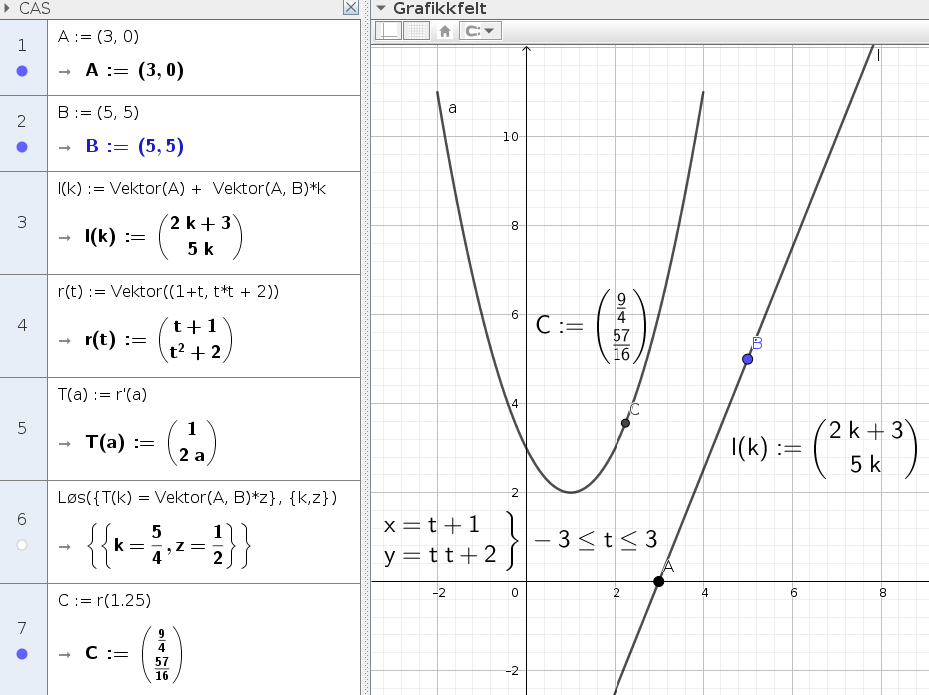
\includegraphics[width=0.9\linewidth]{figs/del2_oppg3}
	\caption{Løsning på oppgave 3, del 2.}
	\label{fig:del2_oppg3}
\end{figure}


\subsection*{Oppgave 4}
\begin{easylist}[enumerate]
	\ListProperties(Style2*=,Numbers=a,Numbers1=l,FinalMark={)})
	# Se figur \ref{fig:del2_oppg4_a}.
	\begin{figure}[ht!]
		\centering
		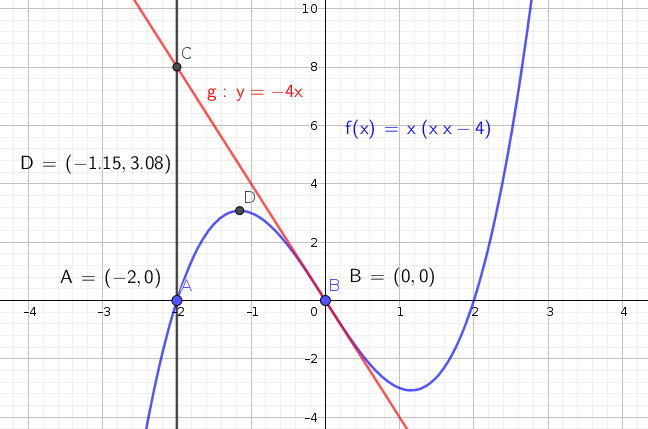
\includegraphics[width=0.9\linewidth]{figs/del2_oppg4_a}
		\caption{Løsning på oppgave 4a, del 2.}
		\label{fig:del2_oppg4_a}
	\end{figure}
	
	
	# Der bruker vi \verb|Mangekant(A, B, C) / Mangekant(A, B, D)| og får $2.5981 \approx \answer{2.6}$ som svar.
	
	
	# Vi argumenterer punkt for punkt. 
	Se figur \ref{fig:del2_oppg4_c}.
	\begin{itemize}
		\item I celle 1 finner vi nullpunktene til $ g(x) $. Siden $ r>0 $, er $ x=-r $ nullpunktet lengst til venstre.
		\item I celle 5-7 finner og definerer vi punktet $ G $.
		\item I celle 8 finner vi ekstremalpunktene til $ g(x) $. Siden $ \left|\frac{\sqrt{3}}{3}r\right|<r$, ser vi av uttrykket til $ g(x) $ at $ x=-\frac{\sqrt{3}}{3}r $ er maksimusverdien til $ g(x) $. Denne kaller vi $ xm $ i celle 9.
		\item I celle 10 finner vi koordinatene til $ H $.
		\item Vi velger $ EF $ som grunnlinje for begge trekanter, som da får høydene $ t(-r) $ og $ g(xm) $. Siden grunnlinjen er den samme, er forholdet mellom arealene til trekantene det samme som forholdet mellom høydene. I celle 11 ser vi at dette forholdet er uavhengig av $ r $, som var det vi skulle vise.
	\end{itemize}\begin{figure}
		\centering
		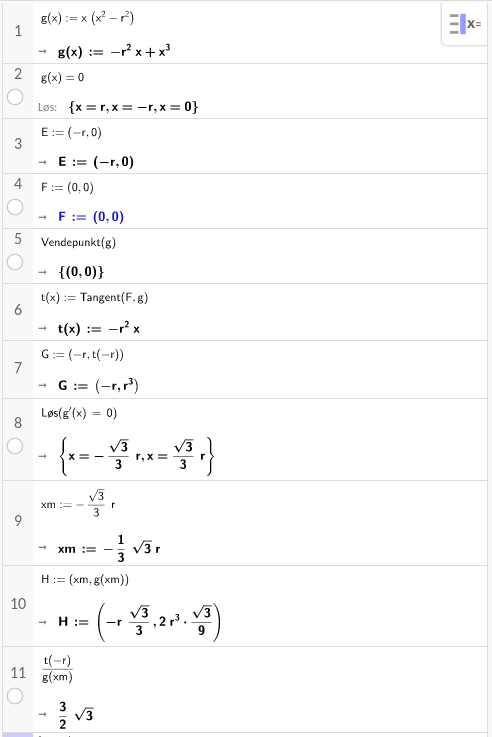
\includegraphics[scale=0.7]{figs/d2opg4c}
		\caption{Løsning på oppgave 4c, del 2.}
		\label{fig:del2_oppg4_c}
	\end{figure}
\end{easylist}





\end{document}